
%(BEGIN_QUESTION)
% Copyright 2006, Tony R. Kuphaldt, released under the Creative Commons Attribution License (v 1.0)
% This means you may do almost anything with this work of mine, so long as you give me proper credit

Identifiser typen {\it filterkrets} (LP, HP, BP eller BS) med følgende frekvensrespons:

$$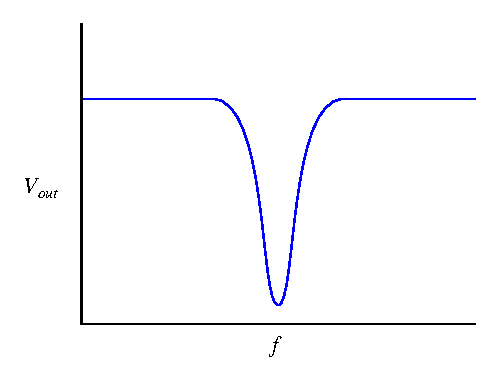
\includegraphics[width=15.5cm]{i00630x01.eps}$$

Skisser deretter et koblingsskjema for en filterkrets som har denne responsen:

$$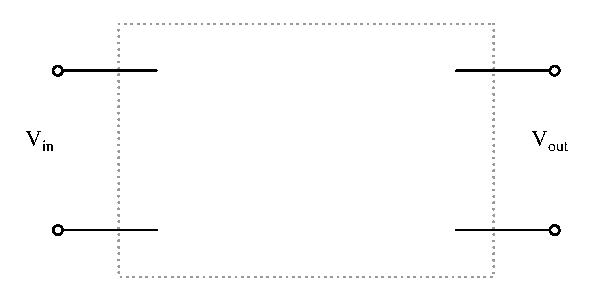
\includegraphics[width=15.5cm]{i00630x03.eps}$$

\vskip 20pt \vbox{\hrule \hbox{\strut \vrule{} {\bf Forslag til sokratisk diskusjon} \vrule} \hrule}

\begin{itemize}
\item{} Finnes det mer enn én kretstopologi som gir denne typen frekvensrespons? Hvis ja, identifiser minst ett annet design som vil oppføre seg på samme måte.
\end{itemize}

\underbar{file i00630no}
%(END_QUESTION)





%(BEGIN_ANSWER)

\noindent
{\bf Delvis svar:}

Dette filteret kalles også et {\it notch}-filter. Du kan selv finne ut hvilken av de fire forkortede filtertypene som er synonym med "notch-filter".

\vskip 10pt

Her er ett mulig koblingsskjema for en notch-filterkrets:

$$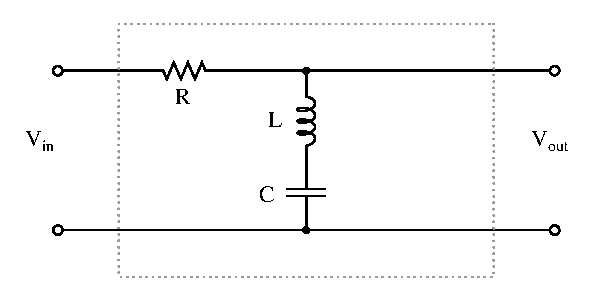
\includegraphics[width=15.5cm]{i00630x02.eps}$$

\vskip 10pt

Oppfølgingsspørsmål: hvordan vil du beregne notch-frekvensen til denne filterkretsen?

%(END_ANSWER)





%(BEGIN_NOTES)

$$f_{notch} = {1 \over {2 \pi \sqrt{LC}}}$$

%INDEX% Elektronikkrepetisjon: filterkrets

%(END_NOTES)
